\documentclass[12pt]{article}

\usepackage[brazilian]{babel}
\usepackage{graphicx}

\graphicspath{{./img}}

\begin{document}

A aplicação distribuída escolhida foi o X.Org.
X.Org é uma implementação do X Window System e
é a base de como interfaces gráficas funcionam no Linux.
O sistema de baseia em um servidor,
ao qual outros programas se conectam
e mandam requisições para que
janelas e outros elementos gráficos sejam desenhados na tela.

Geralmente, o servidor e a aplicação são executados na mesma máquina,
mas é possível, por exemplo,
executar um programa em uma máquina (que seria o cliente) e
o servidor X.Org em outra,
essencialmente virando um sistema distribuído.
Assim, um navegador poderia ser executado em uma máquina,
mas todas as instruções para a construção das janelas
seriam processadas pelo servidor,
que é uma outra máquina.
O protocolo \texttt{ssh} tem suporte nativo para isso,
tornando possível a execução de programas
com interfaces gráficas à distância.

Apesar de haver uma biblioteca para
se comunicar diretamente com o servidor X (Xlib),
isso geralmente é feito indiretamente
a partir de bibliotecas mais simplificadas,
como GTK e Qt,
que têm a grande vantagem de
permitir que o mesmo código seja utilizado em outros sistemas operacionais.

Esse é um bom exemplo de uma arquitetura em camadas.
A aplicação pede a uma biblioteca como GTK
para que uma janela seja desenhada.
O GTK, por sua vez, utiliza a Xlib,
que fala diretamente com o servidor X
para desenhar a janela.
O servidor então vai se comunicar
com o sistema operacional,
finalmente completando a tarefa.

Nesse contexto,
a aplicação, a biblioteca de alto nível, a Xlib, o servidor X e o sistema operacional
são todos componentes com suas respectivas interfaces.

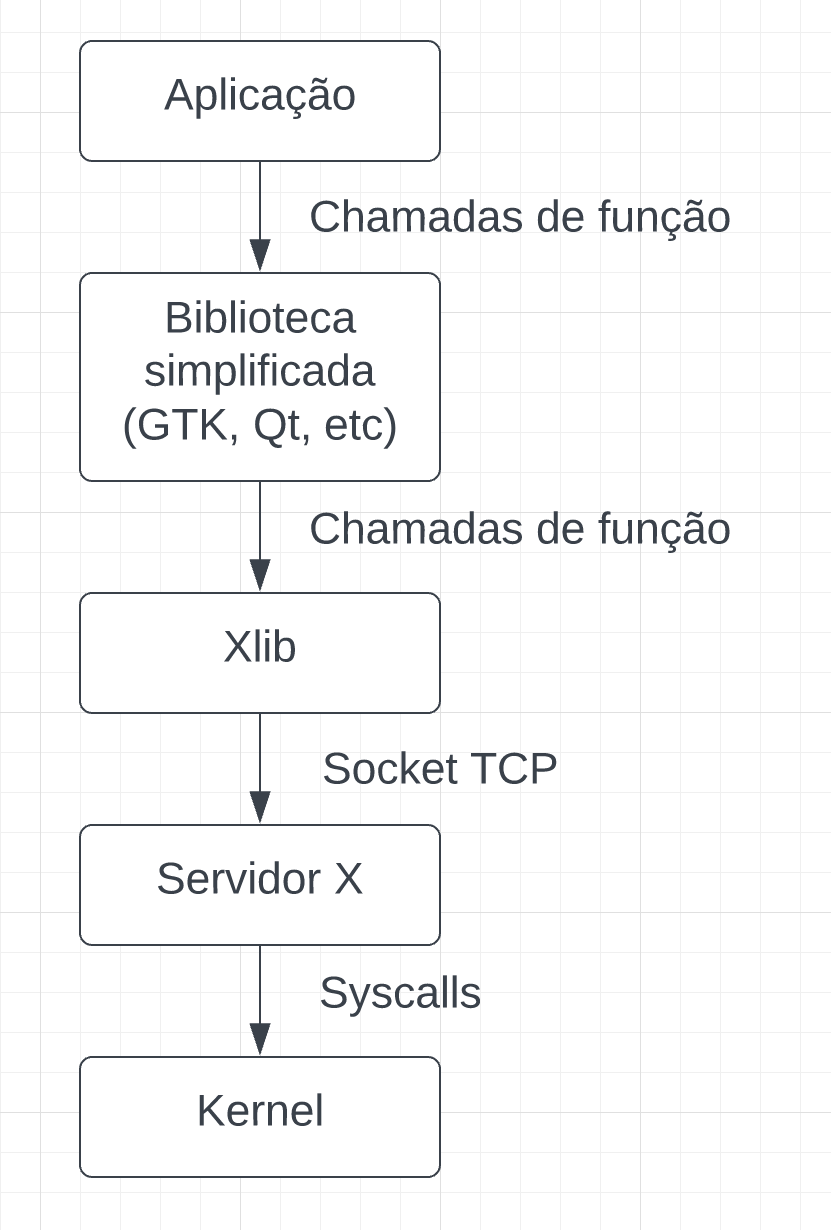
\includegraphics[height=\textwidth]{x}

\end{document}
